\chapter{Introdução}
\label{chap:introducao}

A quarta revolução industrial (Indústria 4.0) é marcada pela integração intensiva de tecnologias digitais avançadas, como a Internet das Coisas (IoT), a Inteligência Artificial (IA) e a computação em nuvem, dentro dos processos produtivos. Esse movimento tem transformado a forma como ativos industriais são monitorados, geridos e mantidos, promovendo um cenário no qual a tomada de decisão é cada vez mais orientada por dados. Nesse contexto, o monitoramento de condição e a manutenção preditiva emergem como pilares fundamentais para a confiabilidade operacional, a redução de custos e o aumento da vida útil de equipamentos~\cite{jardine2006review}.

O conceito de detecção automática de estados operacionais representa um indicador central para a gestão de ativos industriais. Uma classificação precisa dos estados LIGADO e DESLIGADO permite otimizar planos de manutenção, programar paradas de maneira eficiente e calcular o tempo acumulado de operação de componentes críticos. Entretanto, métodos tradicionais para a obtenção desses dados, como inspeções manuais ou sistemas dedicados de controle, apresentam limitações de custo, invasividade e baixa escalabilidade.

Com o advento da Indústria 4.0, tornou-se viável utilizar dados de sensores IoT de baixo custo, que monitoram variáveis como vibração, temperatura, corrente elétrica e velocidade rotacional, para inferir automaticamente o estado operacional dos equipamentos. Porém, a ausência recorrente de dados rotulados em cenários reais impõe desafios significativos à aplicação de algoritmos supervisionados~\cite{cascante2021revisiting}. Este trabalho aborda tanto equipamentos elétricos quanto mecânicos, demonstrando versatilidade para diferentes aplicações industriais.

\section{Motivação e Desafios}

Este trabalho surgiu da necessidade prática de monitorar estados operacionais de equipamentos industriais utilizando dados de sensores IoT. O desafio principal consistiu em desenvolver um sistema versátil capaz de classificar automaticamente o estado operacional (LIGADO/DESLIGADO) tanto de equipamentos elétricos quanto mecânicos, sem a disponibilidade de dados históricos rotulados manualmente.

Inicialmente, foram desenvolvidos modelos baseados em Redes Neurais Convolucionais (CNN) e \textit{Autoencoders} Convolucionais (ConvAE), técnicas amplamente utilizadas em classificação de séries temporais~\cite{li2025hybrid, tziolas2022autoencoders}. A estratégia consistia em gerar pseudo-rótulos através de clusterização K-Means~\cite{zhao2023hybrid}, selecionar apenas \textit{clusters} com alta certeza para treinamento, treinar CNNs com janelas temporais de 30 passos temporais (10 minutos) e implementar detecção de incerteza via \textit{Monte Carlo Dropout}. Apesar de apresentar métricas aparentemente excelentes durante o treinamento (acurácia de 100\%), os modelos CNN/ConvAE demonstraram severos problemas de generalização quando aplicados a dados novos. Os modelos memorizavam padrões específicos do conjunto de treinamento, mas falhavam em generalizar para novos períodos temporais, classificando incorretamente estados óbvios, como períodos com RPM=0 e corrente próxima de zero sendo classificados como LIGADO. Pequenas variações nos dados causavam mudanças drásticas nas predições.

Esta constatação levou à reavaliação da abordagem metodológica, reconhecendo que problemas simples requerem soluções simples. A natureza binária e bem definida do problema (equipamento ligado ou desligado) não justificava a complexidade de redes neurais profundas. Após as falhas com CNNs, foi desenvolvido um sistema baseado exclusivamente em clusterização K-Means, que se mostrou muito mais robusto e confiável. O algoritmo não supervisionado identifica naturalmente padrões nos dados~\cite{habib2015outliers}, permite inspeção e validação visual dos \textit{clusters}, não sofre de \textit{overfitting}, generaliza naturalmente para dados novos, possui treinamento e inferência extremamente rápidos, e é apropriado para a natureza binária da classificação.

\section{Desafios no Processamento de Dados}

Além dos desafios de modelagem, o trabalho enfrentou desafios significativos relacionados ao processamento e qualidade dos dados, especialmente considerando a diversidade de equipamentos industriais. O sistema foi desenvolvido para lidar com dois tipos principais de equipamentos: elétricos (equipamentos com sensores de corrente elétrica, RPM, vibração, temperatura e magnetômetro) e mecânicos (equipamentos com sensores de temperatura, vibração e magnetômetro, sem inferência de corrente e RPM pelo sensor de campo eletromagnético). Esta diversidade de configurações sensoriais exigiu o desenvolvimento de um sistema de detecção automática de tipo e adaptação de processamento~\cite{osornio2023data}.

Os dados são coletados de diferentes tabelas no InfluxDB com frequências de amostragem variáveis dependendo do tipo de equipamento (20 segundos para dados padrão, frequência variável para dados estimados e 2 minutos para dados de \textit{slip}), exigindo técnicas sofisticadas de fusão de dados e sincronização temporal~\cite{tsanousa2022review, tyagi2024comprehensive}. Os dados reais de sensores industriais apresentam lacunas temporais significativas devido a falhas de comunicação, manutenções programadas, problemas nos sensores e interrupções de rede. Lacunas de até 3 horas precisaram ser tratadas através de interpolação adaptativa: lacunas de até 30 minutos utilizam interpolação PCHIP (\textit{Piecewise Cubic Hermite Interpolating Polynomial})~\cite{fritsch1980pchip} com alta confiabilidade, lacunas entre 30 minutos e 3 horas utilizam K-Nearest Neighbors (KNN) temporal multivariado~\cite{cover1967nearest}, e lacunas maiores que 3 horas resultam em segmentação em períodos distintos sem interpolação. Inicialmente, testou-se a \textit{spline} cúbica padrão, que apresentou oscilações artificiais (alucinações) em lacunas maiores, além de redes LSTM (\textit{Long Short-Term Memory})~\cite{hochreiter1997lstm}, cuja complexidade superior não resultou em ganho de qualidade frente ao KNN, conforme demonstrado na Figura~\ref{fig:comparativo_knn_lstm}.

Dados de sensores industriais também contêm \textit{outliers} devido a picos de tensão elétrica, interferências eletromagnéticas e condições transitórias. Foi implementado um sistema de detecção e tratamento de \textit{outliers} baseado no método IQR (\textit{Interquartile Range})~\cite{tukey1977iqr} com multiplicador conservador (3,0), removendo apenas valores fisicamente impossíveis. Para garantir a integridade dos estados operacionais, o sistema utiliza uma regra de proteção de 10 amostras~\cite{habib2015outliers}, que preserva sequências longas de \textit{outliers}, evitando que estados de desligamento legítimos sejam erroneamente descartados como ruído estatístico.

\begin{figure}[H]
    \centering
    
\includegraphics[width=0.85\textwidth]{plots/02_comparativo_knn_lstm_subplots.png}
    \caption{Comparativo entre os métodos KNN e LSTM para reconstrução de lacunas temporais. O KNN apresentou resultados superiores com menor complexidade computacional, tornando-se a escolha definitiva para lacunas entre 30 minutos e 3 horas.}
    \label{fig:comparativo_knn_lstm}
\end{figure}

\section{Objetivo e Contribuições}

Este trabalho tem como objetivo desenvolver um sistema versátil e robusto para detecção automática do estado operacional de equipamentos industriais, abrangendo tanto tipos elétricos quanto mecânicos, utilizando dados de sensores IoT de baixo custo.

A primeira contribuição é a implementação de um sistema de detecção automática de tipo de equipamento que identifica se o equipamento é elétrico ou mecânico baseado nos arquivos de dados disponíveis, adaptando automaticamente o processamento e classificação. Foi desenvolvido um \textit{pipeline} dual de processamento completo que adapta seu comportamento ao tipo de equipamento: equipamentos elétricos recebem processamento completo com corrente, RPM, vibração e temperatura, enquanto equipamentos mecânicos têm processamento otimizado focado em temperatura e vibração, compartilhando técnicas como segmentação temporal, interpolação KNN e Spline, tratamento de \textit{outliers} e normalização.

Uma contribuição importante é a demonstração prática de que soluções simples são preferíveis quando adequadas ao problema, com especial atenção à escolha de algoritmos baseada na natureza dos dados disponíveis.

\newpage
\section{Estrutura do Trabalho}

Este trabalho está organizado em cinco capítulos. O Capítulo~\ref{chap:revisao} apresenta a fundamentação teórica sobre fusão de dados, aprendizado não supervisionado e processamento de séries temporais. O Capítulo~\ref{chap:metodologia} descreve a metodologia implementada, incluindo o \textit{pipeline} dual de processamento para equipamentos elétricos e mecânicos, desde a detecção automática de tipo até a classificação final. O Capítulo~\ref{chap:resultados} apresenta os resultados obtidos com dados reais de mais de 5 milhões de registros de cinco equipamentos industriais, incluindo análise de qualidade dos dados e métricas de desempenho. O Capítulo~\ref{chap:conclusao} sintetiza as contribuições, lições aprendidas sobre adequação metodológica e direções para trabalhos futuros.

A Figura~\ref{fig:fluxo_horimetro} apresenta o fluxo completo do sistema, desde a coleta de dados brutos até a classificação final dos estados operacionais.

\begin{figure}[H]
    \centering
    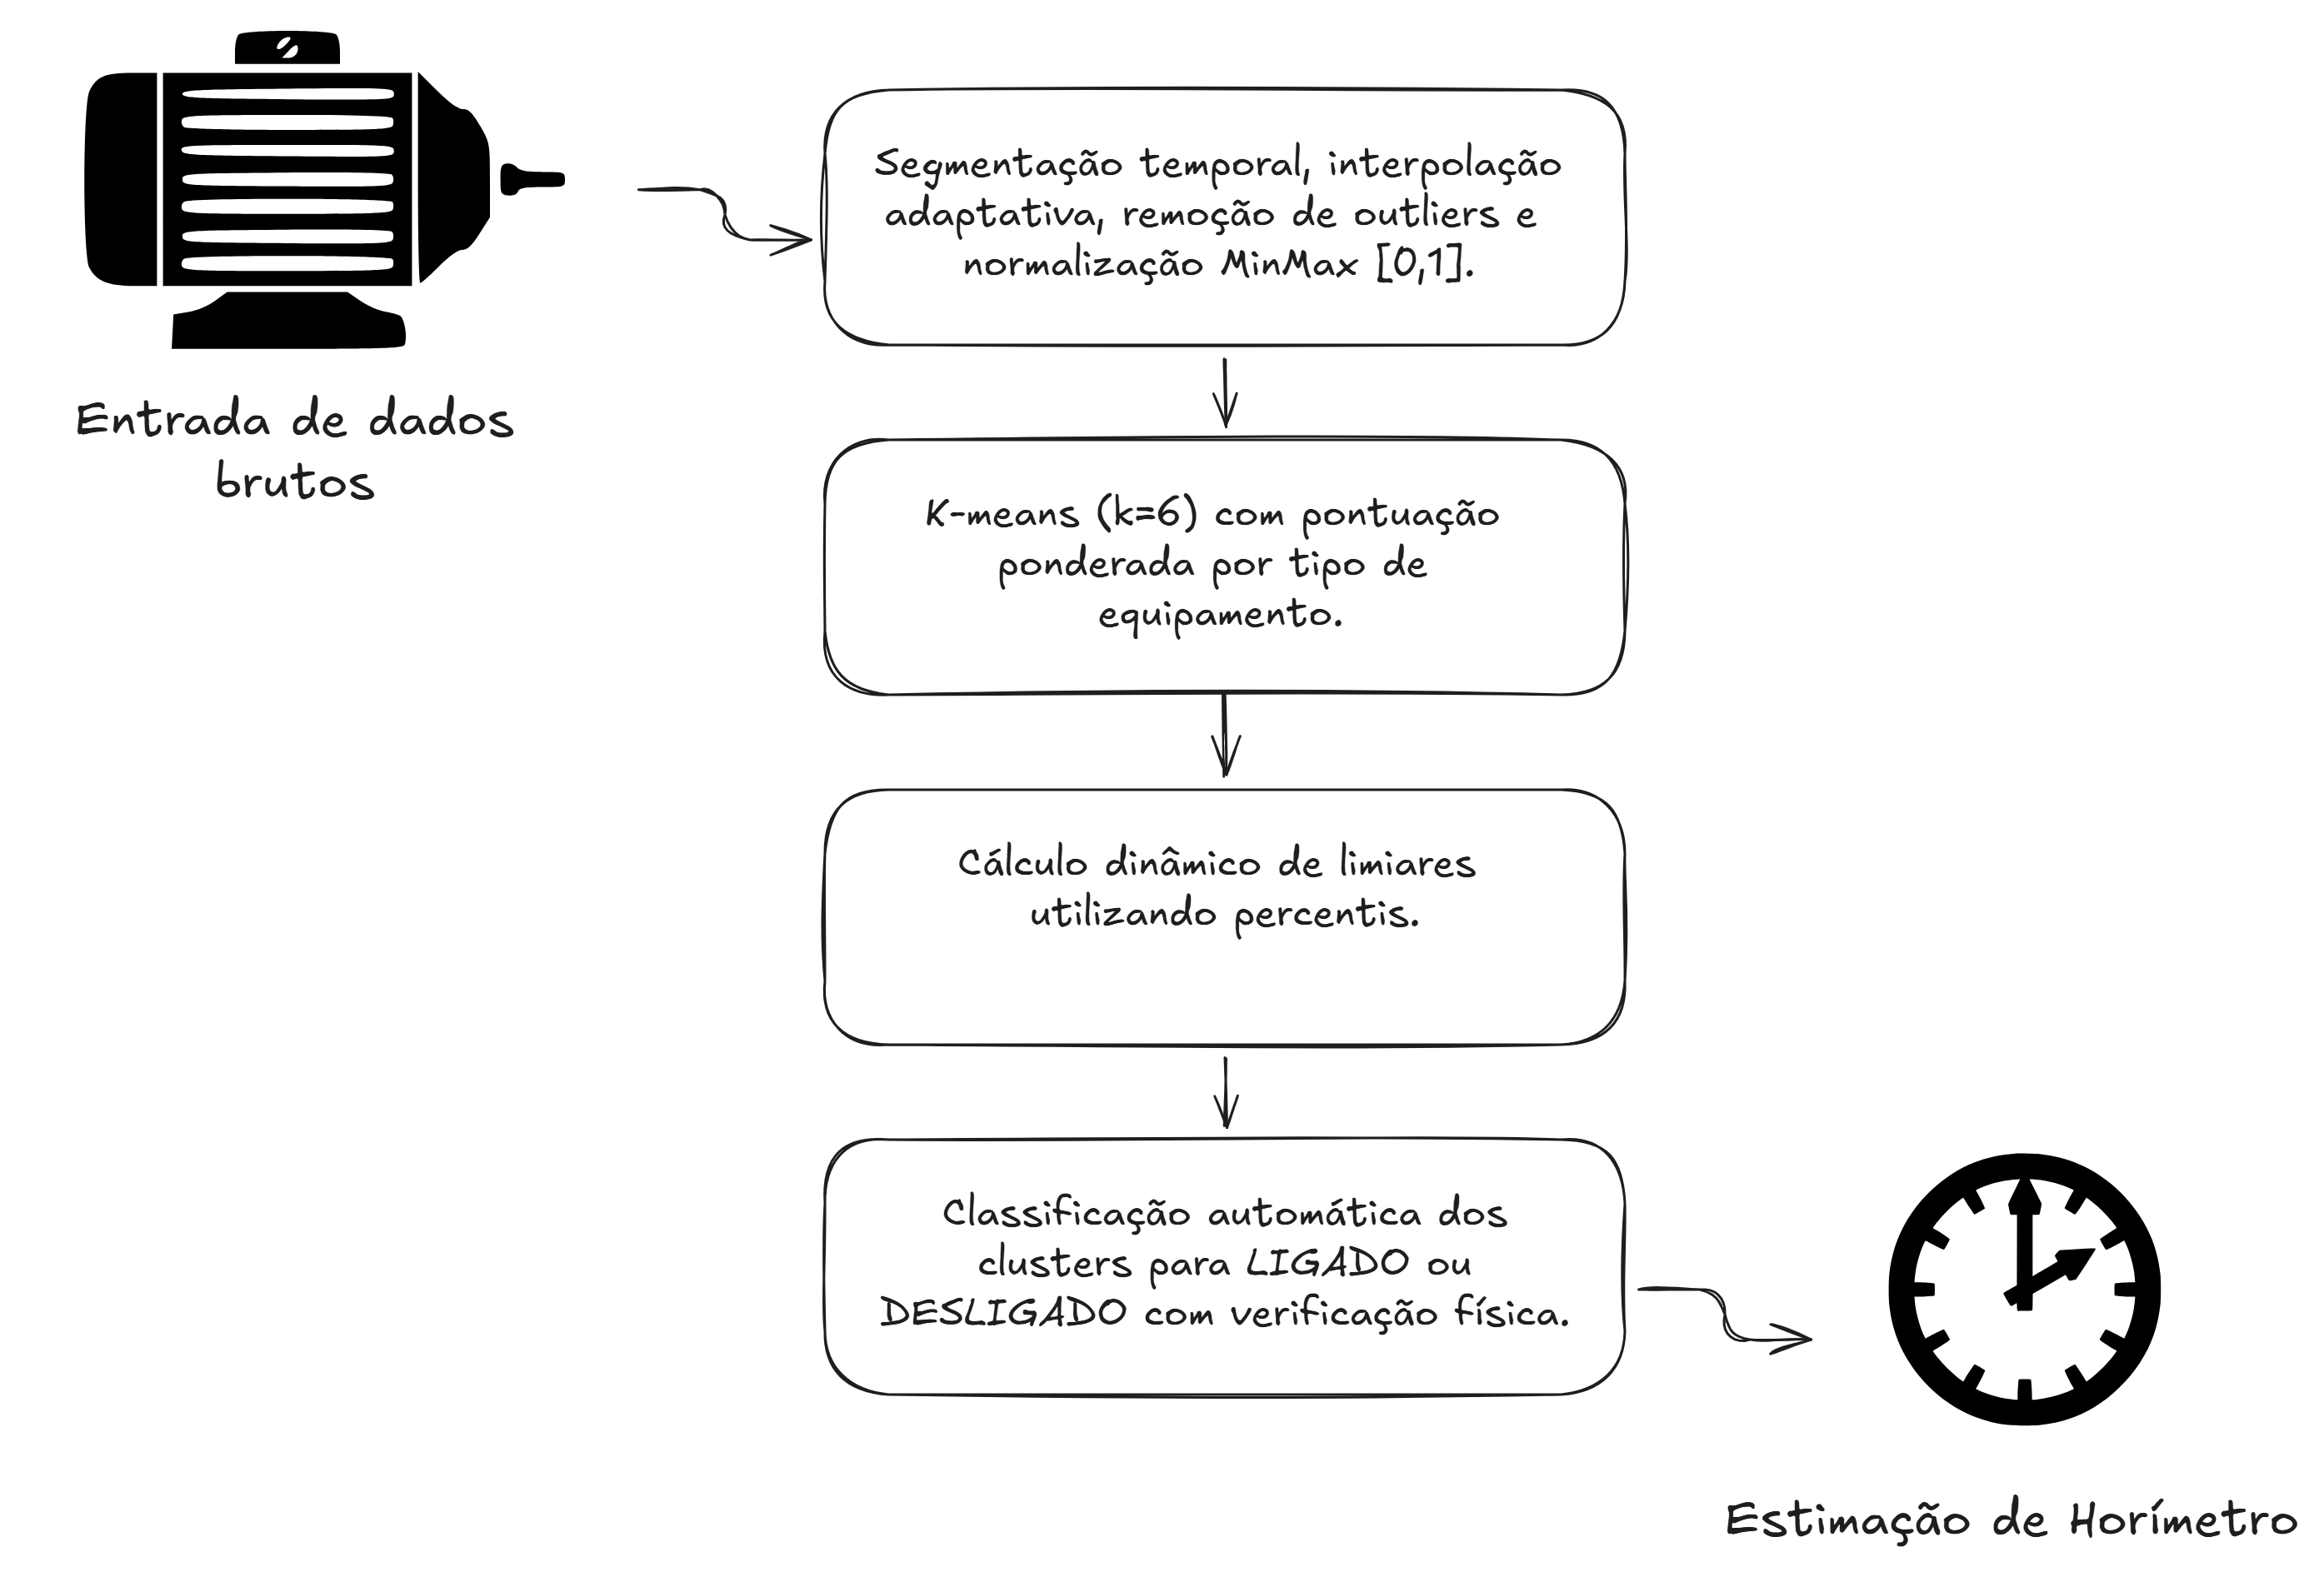
\includegraphics[width=0.85\textwidth]{IMG_TCC.png}
    \caption{Fluxo completo do sistema de detecção de estados operacionais, desde a coleta de dados brutos até a classificação final.}
    \label{fig:fluxo_horimetro}
\end{figure}

\clearpage